\subsection{Questions}
\label{sec:Interviews}

In order for the interview to go smoothly it is important to define the questions beforehand. The questions will be based on the research framework and the evaluation criteria. The interviews will be conducted by Jessie Liauw A Fong and the interviewee will be a software architect.

Questions about how they view software architecture:
\begin{itemize}
  \item What is software architecture?
  \item What is in your company the main job of a software architect?
  \item With which kind of architectures have you worked?
  \item What is the biggest pitfall when implementing a new architecture?
  \item How do you decide which architecture is best of a certain project?
  \item What is the architecture that you implement in most of your projects? (Frontend and backend)
\end{itemize}

Questions about how they view modularity:
\begin{itemize}
  \item What is the first thing that you think of when I say modular architecture?
  \item What are the most upcoming architectures that are focused on modularity in your opinion?
  \item Which programming languages do you think compliments a modular architecture best?
\end{itemize}

Questions about the chosen architecture and method:
\begin{itemize}
  \item What do you think of the image about how I went my way in choosing the right architecture?
  \item What is your opinion about domain driven design
  \item Have you ever heard of modular monolith
\end{itemize}

\begin{figure}[H]
	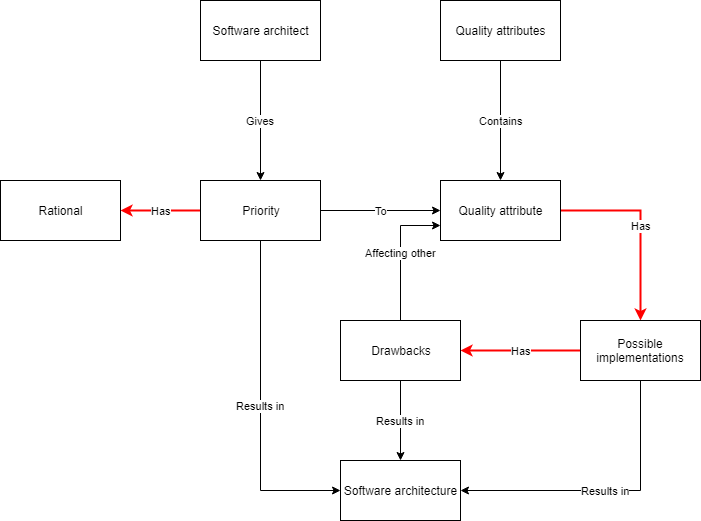
\includegraphics[width=\linewidth]{creating_architecture.png}
	\caption{How a software architecture is chosen}
\end{figure}

\subsection{Interview with Joris}

Jessie: Na mijn eerste vraag aan jou is eigenlijk. Wat is in jouw ogen software architectuur?

Joris: Nou dan hadden weer meteen ook. Heb je een half uurtje?

Jessie: Als je het zo beknopt mogelijk zou moeten uitleggen aan iemand.

Joris: Dan is het sofware architectuur een model van hoe een stuk software geimplementeerd is. Het is een soort abstractie. Als je kijkt naar de architectuur van de auto bijvoorbeeld, de motor bestuur en de deur. Op dat niveau zo kun je ook de software kijken. Software verdeel je ook op een bepaalde manier in min of meer onafhankelijke delen en die delen hebben vervolgens de relatie met elkaar. Dus aan het stuur draai gaan de wielen zo. Als ik software dit hier gebeurt, gebeurt er ergens anders iets anders. En architectuur een van de definitie van architectuur is een soort gedeeld model, gedeeld met engineers en de eigenaar van de software. Over hoe die software nou opgedeeld in brokken en hoe die brokken gezamenlijk werken om de functionaliteit geimplementeerd te krijgen.

Jessie: Ja.

Joris: Korter dan dat krijg ik het niet.

Jessie: Nee dat is een goeie beschrijving. En binnen Ximedes, hebben jullie daar iemand die echt alleen op de software architectuur zit?

Joris: Nee, bij ons is er, vrijwel elk team rol van software architect. Typisch, tegelijkertijd ook de meest ervaren developer. Dus bij ons is de architect ook, die bouwt mee. Meestal wordt er op een bepaald niveau wel iets gedocumenteerd over de architectuur. Met name voor mensen die niet in het team zitten dus opdrachtgevers of mensen die nieuw komen. Ik denk dat in de meeste gevallen de architectuur nog veel meer een gedeeld begrip is binnen zo'n team of dat nou echt een los product is. We hebben ook niemand die alleen maar architect is en niet bouwt.

Jessie: Hoe documentaireserie die architectuur?

Joris: Ja dat wisselt. Ook dat wij werken voor verschillende opdrachtgevers die ook zelf verschillende mensen en eisen hebben. De meeste projecten hebben een document, word document bij wijze van spreken of markdown. Vrije teksten en daar wordt in opgeschreven wat mensen. Het is een beetje een soort cirkel definitie maar daar schrijven op wat het team nodig vindt om op te schrijven.

Jessie: Ja.

Joris: Dat dat wisselt heel erg voor detailniveau. Wat ik altijd deed, ik heb zelf ook gearchitect. Je beschrijft het systeem als geheel met de grove delen is sommige. Sommige stukken ga je even de diepte in. Omdat er bijvoorbeeld iets interessants gebeurt if iets niet voor de hand liggend. Want 9 van de 10 keer zeker bij ons geval wij schrijven code van, typisch project van 40000 regels of zo dus dat moet je. Als je naar kijkt moet je toch wel. Het idee is dat we zulke code schrijven dat als je er naar kijkt je het toch wel snapt. Dus dan hoef je niet helemaal te gaan zitten documenteren.

Jessie: Ja.

Joris: Maar goed daar naast zijn er best een aantal klanten vroeger meer dan nu. Die het heel formeel gedocumenteerd willen hebben. Dingen als uml unified modeling language. We deden het al niet veel en we doen het nu nog minder, omdat klanten het niet meer nodig vinden.

Jessie: En als je dan kijkt naar de verschillen architecturen die binnen Ximedes worden gebruikt. Eelke zijn dat en waarom is daar voor gekozen?

Joris: Ja. Ik denk met afstand de meest voorkomende architectuur is een monoliet. Java of tegenwoordig kotlin, maar een web applicaite op JVM. Die communiceert met relationele databases. En dat of een server sided gerenderde html ui heeft of rich client zoals react, angular of vue die communiceert via de rest api. Ik denk dat dat 80 procent van de projecten zijn. En dat kiezen we omdat we, we geloven er heel erg dat je dingen zo eenvoudig mogelijk moet maken. En dat is een kunst, daar zijn geen harde regels voor maar door de bank genomen is een monoliet voor developers, voor beheerders, voor eigenaars. Eenvoudiger dan een microservices architectuur bijvoorbeeld. En dus als je kijkt naar microservices als alternatief van een monoliet. Dat is nogal wat investeringen die inkomt. Het wordt complex op te bouwen, complex om te deployen. Het lost een hele specifieke set aan problemen op die lang niet elk klant heeft. Voor de de de lood en de performance en de security die wij nodig hebben is een monoliet uitstekend. Dus dat is een beetje de defacto standaard. En wat je vervolgens ziet is dat je per project per klant daarin wordt afgeweken daar waar het nodig is en daar waar het zinnig is. Dus soms worden systemen in 2 delen op in 3 delen of 20 delen opgesplitst.

Jessie: Je wilt je kijkt gewoon naar bijvoorbeeld. Als er 1 deel is wat eigenlijk 9 procent van de loadopvang dan wil je eigenlijk alleen deel onderscheiden.

Joris: Ja, bijvoorbeeld.

Jessie: Dat je die makkelijker kan delen en dat de rest van de applicatie in een instance kan draaien.

Joris: Ja bijvoorbeeld, security is bijvoorbeeld een ander ding. Waarbij je zo min mogelijk footprint service er naar buiten wil laten zien. En 9 van de 10 keer zijn de klanten. Voor developers is er niks handigers dan gewoon een proces wat ik kan starten met dat gedoe en zit je ook weer met je git repositories. Kijk alles schaalt. We hadden ook een project draaien. Die is gestart en die had op een gegeven moment 20 git repositories en die jongens werden dood ziek. Die hebben het nu allemaal in een monorepo gestopt. Dus we zijn continu opzoek.

Jessie: Ja precies ja.

Joris: Kijk en als je facebook bent is het een ander verhaal. Dan heb je een heel team zitten die de hele dag niks anders doet dat repositories managen. Ja zijn we met een mannetje of 4/5 per team zo gaat het.

Jessie: Ja dat snap ik. Oké en als ik het goed heb begrepen hebben jullie wel microservices of hebben jullie wel andere architectuur geïmplementeerd binnen het bedrijf? Wat was de grootste challenge die pitfall die je zag tijdens het implementeren waar je die eigenlijk pas daarna dacht ik van oh ja oké als we dat eerder hadden gedaan. Was het een stuk makkelijker geweest. Of is het vooral tijd dat gewoon?

Joris: Kijk als we even teruggaan naar architectuur als mentaal model van hoe de software werkt. Los even van hoe het deployed wordt, meer aan de binnenkant. Ik kan niet zeggen dat als bedrijf er nou wel of niet iets geleerd is, maar ik heb wel software gebouwd waarvan ik achteraf de dacht. Een goed voorbeeld ik heb ooit software gebouwd voor een lease bedrijf, ING Lease. En dat automatiseerde het verkopen traject. Zo'n lease contract bestaat uit onderdelen, het is een beetje als een hypotheek, je hebt garantor en zekerheden noem het maar op. Complexe gedoe pricing dingen en dat aan de eind van de rit moesten er documenten komen. In het nadenken in het ontwerpen van het systeem. Hebben we heel lang gepraat over dat sales process. En die documentatie was een soort afterthought, oh ja aan de eind van de rit moeten het documenten worden. Ik denk dat letterlijk 3/4 jaar later toen het systeem al heel succesvol was toen merkte we opeens. Toen bleek dus dat er heel veel changes kwamen op die documenten en dat veel mensen ontevreden waren en achteraf. Hadden we met veel meer vooruit die document generatie moeten behandelen. En nu is het een systeem wat contract workflow automatiseerd en achteraf een document maakt. We hadden het als een document generator moeten bouwen die ook wat contractmanagemend deed. Dat is zo'n architectuur dingen waar je later bijna niet meer vanaf komt. Tenzij je het compleet herbouwd. Dat gezegd hebbende. We proberen hier tijdens een project gaat tijdens de bouw heel erg op te letten. Bijna agressief te refactoren als we merken dat het niet meer klopt. Uiteindelijk begin je op een gegeven moment maar te bouwen en dan ga je een kant op, dan heb je een model. En tijdens de bouw merk je. Daarom is het zo fijn dat je snel naar klanten teruggaat, omdat die klant komt met dit bedoelde ik niet. Soms blijkt gewoon dat je een verkeerd zit je domeinmodel. Ja dan los je dat op.

Jessie: Is wat je eigenlijk zegt is dat. En wat je hebt geleerd dat je gewoon eerst gaan kijken van oké wat wat is nou echt het meest grote gedeelte of tenminste de meest belangrijke functionaliteit die de applicatie daadwerkelijk heeft. Waar draait het allemaal om en daar ga je omheen bouwen in plaats van eerst het bouwen, bepalen wat je wilt bouwen en waar je eigenlijk naartoe wilt gaan.

Joris: Hier geloven we sowieso heel erg  ook als wij agile werken. Dan nog beginnen altijd met noem het workshops. Gesprekken met de klant, eerste proof conceptcode. Om een beetje te spelen met de oplossingsrichtingen en daar van tevoren over na te denken. En dat gekoppeld met ijdens de bouw vrij agressief refactoren als je merkt dat het niet goed komt en niet op z'n loop laten gaan dan wordt het een puinhoop. Maar de realiteit is dat je het gewoon ook niet altijd kan voorspellen. We hebben software die soms 10 jaar misschien nog wel langer in productie draait. De wereld veranderd ook in 10 jaar. De software wordt gebruikt voor toepassingen waar ze in 't begin nooit voor bedacht zijn. Dus al heb je het helemaal goed in het begin. De kans dat het over 5 jaar nog matched met waar dan voor gebruikt is, is heel klein. Hoe dan ook is het geen statisch ding. Continu de oplossing vinden bij de realiteit van het bouwen.

Jessie: Dan hebben we het stukje echt over de software architectuur gehad. Nu ga ik wat vragen stellen over modulariteit binne de architectuur. En eigenlijk het eerste wat ik je wat vragen is: waar denk jij aan als ik als ik het heb over een modulaire architectuur.

Joris: Modulair impliceert natuurlijk min of meer ontkoppelde onderdelen, modules. Dus als je zegt modaire architectuur dan verwacht ik dat je het hebt over hoe die bestaat uit onderdelen waarbij het voor sommige onderdelen misschien ook wel meer dan 1 implementatie is. Die dus optioneel zijn. Die je wel of niet hebt. Dat je misschien wel twee of drie versies van dezelfde module hebt. Die je min of meer als een soort legoblokjes inelkaar klikt. Nu vul ik heel veel in op basis van het woord modulair.

Jessie: Dus dat is goed. En als je kijkt naar de modulaire architectuurs die bestaan in de industrie. Welke denk jij zegmaar dat de meeste potentie heeft en daarbuiten ook goed implementeerbaar is als dat een beetje duidelijk vraag is.

Joris: De vraag is wel duidelijk. Ik weet alleen niet of ik er wat zinnigs over zeggen. Kijk dat had ook te maken met mijn achtergrond. Wij bouwen maatwerk software in opdracht waarbij we elke keer met een wit vel beginnen en zelden hoeven rekening gehouden met het feit dat dezelfde software bij het meer dan een klanten draait bijvoorbeeld. Waarbij dus ook zelden de noodzaak is om echt dingen plugable te maken. Dus in die zin heb ik er niet heel veel ervaring mee. Ik weet wel dat voor ons de paar keer dat we hebben geprobeerd dit te doet het altijd erg tegenviel. Moeilijk is om het goed te doen. En goed nogmaals voor ons de return on investment er bijna nooit was om dat in de praktijk werd module a nooit vervangen door module b. Ik heb wel eens nagedacht over plugins enzo. Het lijkt me verschrikkelijk moeilijk om in een keer goed te doen. We hebben wel een beetje ver van weet want we doen het eigenlijk nooit.

Jessie: Ja en als je kijkt naar de, dit is veel meer low level. Als je kijkt naar de programmeer talen. Welke programmeer taal denk je dat het beste modulariteit complementeerd, modulaire architectuur. Als je denkt aan die plugins.

Joris: Ik zou in ieder geval naar een statisch getypte taal gaan. Dus Java, C\#, Kotlin noem het allemaal maar op, maar niet javascript, want je wilt wel echt. Ik 1 van de dingen die je natuurlij heel strak moet hebben in een oplossing is het interface. Is het contract tussen 2 modules.

Jessie: Ja.

Joris: Een deel van dat contract zijn je types. Welke berichten gaan erover en wat zit erin, wat is optioneel, wat is een string, wat zijn de validaties op die string. Als je kijkt naar code, als je dat contract wilt uitdrukken in code. En dan zou ik helemaal gek worden als ik daar geen getypte taal gebruik. Het alternatief is natuurlijk dat je interfaces gaan over het netwerk gaan. Het is dan altijd REST of SOAP of van die dingen. Dan maakt de taal natuurlijk weer minder uit. Binnen de getypte talen zou ik niet 1 2 3 een soort voorkeur hebben dat de ene taal geschikter voor dit soort architectuur dan andere.

Jessie: Misschien ook framework specifiek?

Joris: Ja ik denk dat je meer richting de frameworks gaan. Zeker aan de javascript kant. Dingen als spring

Jessie: KTor?

Joris: Ja KTor. Dat gezegd kotlin kent ondertussen wel contracten. Contracten gaat nog een stap verder dan types bijvoorbeeld een onderdeel van wat je tegenwoordig in kotlin kan uitdrukken. Als je deze functie aanroept, dan komt er altijd een positief integer uit. En dat gaat verder dan zeggen een integer. Ja want want er is geen type in kotlin die positieve integers typed dus je hebt meer nodig dan alleen maar de types dus daar zou je nog naar kunnen kijken maar dan praat je heel erg over sdk level. En ik denk eerlijk gezegd dat het hangt van je van je project af. Als jij een plugin structuur hebt waarbij je bij runnende code, code injecteert. Ja ,dan heb je het over dit soort dingen. Als je het hebt over modules die via het netwerk communiceren dan maakt het eigenlijk niet uit.

Jessie: Dat is natuurlijk ook een van de krachten van microservices, dat je niet overal dezelfde taal hoeft te gebruiken.

Joris: Ja, exact. Dat je polyglot kan zijn. Dat je het aan de verschillende teams over kan laten.

Jessie: Dat was het stukje over modulariteit. Ik heb zeg maar een architectuur gekozen. En ik heb daarr deze eigenlijk een soort van flow diagram bij gebruikt. De Rode lijnen heb ik onderzocht. Wat ik eigenlijk heb gezegd is een software architect geeft prioriteiten aan een quality attribute. Die quality attributes zijn door ISO 25010 gedefinieerd. Die quality attributes hebben mogelijke implementaties. Al die implementaties hebben mogelijke drawbacks. En uiteindelijk doormiddel van je prioriteit te koppelen met die drawbacks kom je uit op een software architectuur. Mist er iets in dit plaatje of zeg je als ik een software architectuur kies kijk ik er anders naar.

Joris: Ja, dit is wel aardig bedacht. Ik denk zelden in dit soort formele termen, maar kijk waar ik het wel heel erg mee eens ben is dat architectuur een afweging is tussen verschillende belangen die die onder spanning staan. Security performance begrijpelijke code noem maar op.

Jessie: Allemaal dingen die je uit de ISO 25010 komen.

Joris: Ja die hebben het ook vaker gedaan. Kijk een andere definitie van architectuur zou het zou zeker kunnen zij precies dit. Een gewogen afweging van wat we voor een stuk software wat prioriteit geven en waar we dus de pijlen laten vallen. Dus als je zegt ik ga 100\% voor performance. De kans dat je leesbare code krijgt is de lager en andersom ook. Dus in die zin vind ik het een mooi plaatje. Alleen het zegt meer over het proces van hoe kom ik op een architectuur dan de architectuur zelf, maar dit klinkt heel redelijk.

Jessie: Dan is mijn volgende vraag, ik neem aan dat je weet wat domain driven design is?

Joris: Ja

Jessie: Wat zijn jouw gedachtes erover? En hoe, als je dat implementeerd. Hoe implementeer je dat binnen Ximedes?

Joris: Ja hoe heet die man ook alweer? Erik Evans? Ik heb ooit een boek gelezen en ook een workshop van hem gehad. Dus ik vind dat ik vind de ideeën heel interessant en ik denk ook dat er. Ik had het een tijd geleden over die workshops die we altijd doen. Hoewel we bij Ximedes nooit dus echt domain driven design volgens het boekje hebben gedaan. Merk je wel dat, een belangrijke uitkomst van zo'n workshop is inderdaad zo'n gedeeld domeinmodel. Gedeeld besef van hoe een subset van de wereld werkt. Neem mijn lease software van daarnet. Dat is een complex ding, met contract, pricing, scenario en dat soort dingen. Een goed deel van die workshops simpelweg bedoeld om developers te laten snappen hoe die businees werkt. En ook een beetje om die business te laten verslappen wat de beperkingen van de implementatie van software. Als dat zo doen kun je dit wel, maar dat lukt niet. Dat vind ik wel echt heel mooi. Wat wat we naar mijn weten nooit gedaan hebben. Is dit zo formeel als Erik Evens het bedoeld doorgetrokken naar de implementatie? Wat ik een interessant idee vindt van hem is dat je zegt van ja, dat mag. Dus zoals ik het me nog herinner, tijd geleden, kom ik tot het domein model en dat komt 1 op 1 terug in de software en is ook 1 op 1 hoe je requirements uitdrukt. Ja ik vind het een prachtig idee, heel formeel. Wij doen het niet. Ik heb het ook nooit gedaan dat. Ook hier zie je met al dat soort dingen zal d'r een.

Jessie: Het is een heel groot verschil tussen tussen theorie en implementatie?

Joris: Nou ja en d'r zitten voor een redelijke mate van compleetheid in. Ik snap ook in het boek natuurlijk een soort extreme maar in de realiteit ga je nooit helemaal naar dat punt want het de return on investment wordt steeds lager, maar ik denk dat we dat als Erik Evans naar onze workshop zou kijken dat hij wel redelijk tevreden was. Als je naar de code kijkt een stuk minder. Een consequentie van domain driven design helemaal doorvoeren naar de implementatie is dus dat je ook al die bounded context dingen en dat dat is wel heel. Onze software is gewoon simpeler. Wij vallen toch heel vaak terug op. Ik heb objecten en ik heb value objecten dus objecten waardes in zitten. Ik heb een service laag waar ik methodes op kan aanroepen. Dat we dan weer documenteren en ik heb wat lijm tussen die dat allemaal aan elkaar zet. Dat is geen domain driven design maar het werkt wel lekker.

Jessie: Als ik me goed kan herinneren heb ik aan jullie eigenlijk 2 implementaties. Eentje was eigenlijl layered architecture, maar jullie deden ook wel iets, ook domain driven design. Dat je 1 package had die over een domain ging.

Joris: Ja. Ja we hadden met name 1 architect. Die is weg, maar goed dat heeft hier niks mee te maken. Ja ik heb daar heb ik altijd wel mee geworsteld. Ook dat vind ik het heel idee. Alle software die ik bouw is altijd gelayered.

Jessie: Ja ja, precies

Joris: Waar ik altijd naartoe neig. Vervolgens als je het 1, 2 keer abstracte trekt. Heeft het te maken met die keuze. Java software maar ik denk elke software in de wereld valt in eerste orde uiteen in een aantal noemen het packages, noem het, maakt me niet zoveel uit wat je kiest. En wat je altijd ziet. Wat je ook kiest. Daar zullen altijd concerns zijn. Quality attributes in jouw plaatje. Die daar dan vervolgens niet lekker in passen. Als ik een layard architectuur maak. Dan is een gegeven stuk functionaliteit vanuit een use case verdwijnt opeens door allerlei verschillende plekken en allerlei verschillende lagen. Als ik zeg mijn primaire modules zijn mijn use cases. Dan vallen andere dingen weer een beetje in het niet. Bijvoorbeeld de database logica zit dan ineens op allerlei plekken tegelijkertijd. Hoewel ik het. Ik vond het een heel interessante dat een keer wat anders dan dan dan klassieke three tier layered. Maar het zal ook hier weer per project. Ook hier moet je weer een keuze maken. Eigenlijk heb hier ook weer architectuur te pakken. Hoe je dat een gegeven project een gegeven klant gestructureerd. Het hangt ervan af. Ja, het is ook dat je je hebt ook heel erg hebt te maken met de verwachting van een engineer die over 5 jaar op je project zit. Ik kan natuurlijk heel wild gaan en zeggen ik ga het allemaal anders doen vandaag. Maar dan optimaliseer je niet voor die arme ziel die opeens bugs moeten gaan zitten fixen. Dat zit ik ook wel heel erg mee. Het zijn lastige dingen.

Jessie: En? Heb je wel eens gehoord van een modulaire monoliet.

Joris: De term hoor ik vandaag voor eerst.

Jessie: Oké dus. Snel uitgelegd. Het is eigenlijk domain driven design. Dus je hebt eigenlijk verschillende lagen en dat zijn allemaal domains. Die praten met elkaar over dezelfde api. Bijvoorbeeld:  User of employee heeft een shift. Dan heeft een shift een many to may relation met een employee. En die many to many relationship wordt gedefinieerd via het interface van employee. Employee heeft een interface en daarom weet shift welk moedle hij moet gebruiken. Elke module dus die exporteert ook altijd maar 1 model. En zo heb je eigenlijk de toevoeging dat elke module kan in een aparte repositories worden gedeveloped, door aparte teams. En die kunnen on build time bij elkaar komen. Snal je een beetje wat ik bedoel?

Joris: Ja, maar jouw voorbeeld als ik een shift module maak. Ik moet wel een concept van employee kennen. Is dat mijn eigen implementatie of moet ik op compile time de employee module kennen?

Jessie: Het kan op compile time. Als je niet als je niet met een compiled taal gebruikt.

Joris: Ja precies, ik moet wel het employee concept kennen?

Jessie: Ja klopt, je kent het employee concept. Hetzelfde als dat eigenlijk microservices werken. Je moet weten dat er een andere microservice is die een bepaalde actie ondersteund, maar het interface of de rest api is hetzelfde als bij andere microservices. In plaats dat je een interface hebt over de daadwerkelijke rest api of graphql of whatever. Heb je het nu over de code. Hoe je praat over de code. Een voorbeeld in spring is dus bijvoorbeeld als je dus verschillende layers hebt dat je dan een nieuwe jpa object implementeerd en dat je daarin meteen kan zeggen api.employees is de foreign key. Dus het model wat gekoppeld wordt. Dat is dus wat ik heb gekozen en ik wou je eigenlijk vragen: Wat is je eerste reactie hierop als je dit hoort? Als het nog niet duidelijk heb ik ook een code voorbeeld.

Joris: Het is half duidelijk, maar los daarvan. Mijn vraag is eigenlijk welk probleem los je op? Het klinkt complex en meer werk dan alles gewoon in een monoliet gooien. Dus waarom doe je dit?

Jessie: We omdat het idee is dus als jij. We hebben 1 basis applicatie en laat zeggen er een hele grote klant naar ons toe, maar die wilt 1 module anders hebben. Dan kunnen we nu zeggen oké we bij switchen die modellen switchen gewoon om. Want dat is nu mogelijk omdat je dus omdat ze sowieso over dezelfde api praten kan je ook gewoon een hele module eruit halen kun je de nieuwe module erin stoppen. De applicatie werkt vanzelf nog steeds het zelfde.

Joris: Maar de beperkingen zitten in je api. Daar zitten je grenzen van je vrijheid.

Jessie: Misschien ook wel weer een. Omdat die is maar 1 model mag, leveren eigenlijk. Het geeft wel weer een soort van. Je moet er wel weer meer nadenken over de architectuur voordat je eigenlijk zo'n module begint. Je moet deze wel geaccepteerd worden. Als er maar 1 model wat wat dit model gebruikt moet het dan wel een hele eigen module worden, ect, ect. Dat zijn eigenlijk de afwegingen ervan.

Joris: Ja precies.

Jessie: Dat is eigenlijk waar ik ben gekomen. Dus als je dit even snel hoort wat zijn je eerste reacties? Hoe denk jij erover?

Joris: Nou ik denk dat je over de goeie dingen druk maakt. Als je zegt, laten we zeggen dat wij meegaan met je uitgangspunt die modulariteit nodig is. Daar heb ik geen mening over. Als het nodig is dan maak je, je over de goeie dingen druk. Ja ik weet te weinig van het domein om een verdere mening of dit wel slimmer is dan iets anders, maar het klinkt wel heel redelijk. Wat ieder geval klopt naar mijn gevoel is dat je zegt. Je maakt planning software toch? Daar gaat het om. Kijk linksom of rechtsom. Nou je zou nog een case kunnen maken. Beperk je nou niet teveel tot de plannen van de employees. Maar dat zijn precies het soort ideeën natuurlijk waar je over moet nadenken. Kijk software die alles kan kun je niet verkopen want die doet niks. Dus je moet een soort toepassing hebben. En daarbinnen weer zoveel mogelijk verschillende klanten kunnen bedienen zonder dat je allerlei if statements moet doen. Ja, dat vind ik heel goed en ik vind het een interessant idee om dit pluggability mogelijkheid te combineren met een soort domain driven design analyse. Waar lopen mijn entiteiten nou. Dat vind ik eigenlijk wel heel slim ik heb daar nooit of zo. Ik heb die 2 dingen nooit gecombineerd in mijn hoofd.

Jessie: Dat is dus het onderwerp van mijn scriptie.

Joris: Ja dat je een heel goed onderwerp te pakken hebt. Ja leuk. Goed idee.

Jessie: Dat was eigenlijk dat waren eigenlijk al mijn vragen. Dankje wel voor het interview

Joris: Ja graag gedaan. Niks leukers dan lullen over het vak.

Jessie: Dat vind ik dus ook.


\subsection{Interview with Dimitrios}

\subsubsection*{Information}
Name: Dimitrios Parrou
Email: dimitrios@endouble.com

\subsubsection*{Interview}

Jessie: Hello Dimi. So right now I'm writing my thesis to finish my bachelor's degree. In software engineering and my subject has a lot to do with architecture or it is. It is architecture. So that is why I came to you and I want to ask some questions about software architecture. So the first one is big. So what do you think software architecture is.

Dimi: There are official definitions and there are so many actually that basically I'm pretty sure no one will give you the same definition. But for me software architecture is when you think of a system how it's organized the relationship between the components you know how the application is deployed. All the principles that guide know the building and the design of the application.

Jessie: So if I'm understanding it correctly it's more like an abstract layer that is just above code. So if the actual code and then you have the architecture to right above that and then make the design above that again.

Dimi: What do you mean design?

Jessie: So you have software design and software architecture. Do you have a difference in those definitions or?

Dimi: The thing is that. Well first I to comment on. You said it's a level above like abstract level. I do not consider it as a level. Well maybe if you look at it like you have to start somewhere. You cannot just start something with that right. Because you really need to have a plan. You cannot just go build something blindly. Then again then the thing is that so we're literally splitting the collection of the principles like that those guidelines. And if you compare that with buildings you know you know the architects already would create this plan that looks and plan with their civil engineers will take and then start building them like the rest. This plan is basically software architecture.

Jessie: So in Endouble. What is the main job of a software architect. Well what what is a day to day job.

Dimi: Well we do not have a dedicated role in Endouble and that's why you have me which is basically the next round of CTO and software architect because I have the background. But usually what what we do is you know you work with this. We delegate to the tech leaders. You know you take that it takes a decision which they do that together with me when we discuss it and then you know tech leads meeting. So what does an architect do usually in Endouble? The architect ensures that he balance the non-functional requirements and the company requirements at the same time. For example you have you know you have clients that have some requirements that their website needs to be performing. It has to be able to handle that amount of requests per second. It has to be robust. You know the architect still in Endouble has to make sure that their applications can satisfy those requirements. But at the same time they satisfy the company requirements which are meant to make it easier, you know, to understand all this kind of stuff.

Jessie: So they they're balancing so just to go back to the definition of ISO, ISO is given the 25010. I do not know if you're familiar with the quality attribute. Yeah. So what you're saying is that the software architect balances the requirements of the company with the quality attributes.

Dimi: Yes but with a special focus on the non-functional requirements

Jessie: Yes exactly. So what kind of architectures have you worked with?

Dimi: Of course the one known to all of us: the monolith. We have build the layer architecture which is that you know sometimes you know it has MVC. Pretty common in web applications. I have worked with service oriented architecture and I hate it. Microkernel you know?

Jessie: No I do not know microkernel.

Dimi: you know when you have a word with thinking. You really know it. I am gonna tell you later about it. Of course I work with them in micro services which I love. Event Driven Architecture. Yeah. Very very fond of that thing and space based. You also have worked with space based and pipes and filters is something I work with, with my personal projects, which i really love. And serverless but only experimenting. I do not have work experience with it.

Jessie: So space based and microkernel. Those are the two I am not familiar with.

Dimi: So microkernel is basically when you have a let's say common core and on top of that you can enhance it with other kind of modules. If you look at wordpress, it is exactly that. It has a kernel, something that you can see as the core and than you can add more.

Jessie: Ah that is what CSB is build on right?

Dimi: Exactly. But that is the thing about microkernel. And the thing in your questions you had written modular monolith. I wasn't familiar with modular monolith. But what you mean is actually the microkernel. It is a monolith that is modular and that you can extend.

Jessie: I could not find the official term.

Dimi: Microkernel is the official term.

Jessie: To bad I found out so late it is called that.

Dimi: The thing is that all that stuff like I also wasn't familiar with the official term and because we know you learn also by experience and I think the software architecture of o'reilly where I go. I am a veteran there. I know all of them. Since 2015 I go there. This is where I meet all the great architects and where I hear about it all standard, official terms. That is also where I learned space based. You know it because space based is nothing more than you know when you scale horizontally.

Jessie: So mircoservices is also space based?

Dimi: Kind of. Microservices has a different principle.

Jessie: That is quite a lot of architectures. So you of course have a lot of experience implementing these architectures. And because you have implemented so many what was the biggest pitfall that you saw with most with most of them. Yes. Did you underestimate the certain thing multiple times or what. Yeah. What was the biggest pitfall.

Dimi: I will tell you. Not only are you asking me when I implemented those but also when I saw to my team members implement them?

Jessie: Both!

Dimi: Well I think the biggest one is when you pick an architecture that satisfies in requirement that it's not there. This is pretty common from developers that I've seen when you know they want to pick an architecture because it is more performant or faster or whatever but you were never asked to make it more performant. And now when you do that you bring all the complexity of that architecture that solves the performance. That it was never there. You have to deal with all the complexities. That's that is for me the number one pitfall.

Jessie: What most of the times happen when people are implementing microservices.

Dimi: Yes but there is also a way to make microservices simple. So you do not have to go out of your way. But than again that is the thing. Well I think the next question is. How you decide.

Jessie: Exactly. So the let's first jump in. The better question would be then so yeah How would you decide what architectures best for your current application as you said. You have to. You have to take into account these these quality attributes but how do you go about your way in doing that.

Dimi: So what I would do is first of all I get together the requirements and there are two places that I can gather that first places the client. So the client will tell me what exactly they want and I have to go and ask them the important questions about the non functional requirements in terms of security, scalability, redundability, robustness. This kind of stuff and performance of course. Well these are you know what are important for their client. And at the same time I have to take into account the company requirements. And this is what some people actually forget to do. What are the company requirements. The company requirements are maintainability of course easy to understand. Easy to add code or remove but one more thing that people tend to forget is they do not take into account the capabilities of a company. So if your company does not have the experience how can you go on and take an architecture that requires that. Right now even with microservices. Even though they are very simple. And if you think of them alone as services if you think about it the infrastructure that you need to make them communicate to make them deployed in that kind of stuff. It requires a lot of devops work. And if your company cannot afford it. Either because it doesn't have the experience or because it does not have the capacity right then it's wrong to pick that architecture. This is what you have to balance. You take those two a let's say a sources of non-functional requirements and then you pick the best that balances. Thats how you go.

Jessie: Yes that sounds good. So which architecturally do you prefer implementing and probably. Again it is requirements specific. So I will give an example of what I'm implementing and maybe you can give you a rationale or what you would implement of course you do not have the full picture but yeah. So right now I am building an application, EFFE, it is planning software for employment agencies. You have a main application, so you have a main application which has basic functionalities. But there is a possibility that big client comes in. He says Okay I want these basic functionalities changed. I want that a user has an extra field, when I save user should be called to my to another system et cetera et cetera. There's a lot of requirements. It should be very modular much I mean maybe the is not the best word. Flexible. Flexible it should be very flexible in order to have the basic function of basic application but also the application that is more catered to a certain client that will pay more. And then the question is how would you. Which architecture do you think it's best for backend and frontend.

Dimi: So basically what's you said right now it's a pretty typical application. But you didn't mention any of the non-functional requirements. Which are the ones that dictate. But anyway I can already understand from your case because you are the sole developer. So immediately having unpacked some equipment there you need to be able to have enough time to maintain that so it doesn't think you for life. So you can do other stuff you can enjoy your life.

Jessie: Well actually. So my the first thing I did with my thesis I was ranking quality attributes and what I found most important and I can give you here the quick recap the first one is maintain ability. The second one is compatibility. Third one is functional. Sustainability security reliability performance portability usability because yeah performance is not really important for us/

Dimi: Social performance is subjective like. You would notice that in web applications performance doesn't really matter much. It would not matter and I do not know maybe the voting applications where you really have.

Jessie: Yeah okay. So in your opinion what do you think. Yeah. Talk to just tell me what what you take in and how are you...

Dimi: Will tell you how I would approach it. For more of those architectures. There's always something that I am leaning towards and I can already tell you that of course for me microservices is the way to go. I'm fairly convinced about that and actually love the whole idea. But they will not pick it for the simple project or a small project, right. Because of the overhead that it requires in terms of your devops and a lot of other stuff that I have to put myself in. I learned how to do it. Yeah. So I can do it and I'm doing it for my project but it's a pain in the ass. And then what I would do is try to make scaled down versions of that for example if you think about the whole microservices that you keep a one set of service independent of each other right. You can even structure that in one you know even in the monolith or you know in your backend as different packages and those packages have their own migrations, their own configuration, their own classes and everything there and you know for connections, drivers and they can potentially be taken apart and be deployed independently in another you know service but it's fine if they live, at the start of the project, there. And they can maintain it easier. I can test it also easier because the important part is that by the time you want to switch to microservices you're testing should already be in place and the testing difficulty increases as well. Because of this decoupling that is there. However when it is on the same application the existing tools that we have are pretty good. So if you take advantage of the principles of microservices but say in one application for starters for me it is always the way to go. But I have also some rules like if it's a website that you need to build it MVC I will pick that because it's a proven way. There is no need to go microservices for a website.

Jessie: Okay. Yeah. That's so so what you recommend is then micro kernel or/

Dimi: I would not go for a micro kernel at the start. Making sure it is a separate library or package or whatever you call it, is independent and decoupled from the rest. And this a micro kernel gives me at all times at times the possibility to take it that way and have it as a depedently deployable microservice. So I get best of both worlds.

Jessie: Yeah and you get you get to decoupling and the encapsulation of microservices.

Dimi: Yeah. So if there is a new requirement that comes in for let's say performance or something then you can scale up. But why you do it from the start. You know pay all of the cost.

Jessie: Exactly. OK. So yeah that was my. There was. These were the questions a bit more about server architecture. Next few questions will be about modularity. Yeah. So yeah. The first thing what comes up to you when I say modular architecture

Dimi: When I hear modular the first thing is decoupled components. With anything that might include to either independently deployable or not. Then the whole idea of building modular that is not its decoupled and you can replace it.

Jessie: I think we already touched upon this a lot but your opinion the most what are the most. What are upcoming architectures that are focused on modularity.

Dimi: I can tell you already microservices is the king. Yeah it's proven now. You would see a lot of buzz last year on the conference. Yeah but now it's pretty standard. There is no better thing for him than microservices because microservices give you not only the ability to have components you can replace. With anything else at all times it gives you the ability to have your own whatever language you want, whatever datastore. Whatever services. It does not matter. So the king is microservices. But then if you ask me about upcoming architectures then you should already know about the evolutionary architecture right.

Jessie: No I haven't heard of.

Dimi: Yes evolutionary is a term I first heard two years ago at the software architecture conference by neal ford. Very great guy and everything and he's been doing talks on that since then and the whole idea of evolutionary architectures is that you build an architecture that really aligns with the days agile and everything. The main problem sentiment was that when you built an architecture. Systems evolve, systems change. You can never beforehand think you're the best structure for what is gonna come. You do not know. So what do you do is you make enough architecture that can support your and a little bit towards the future needs and then you build on top of that. But how do you sure of that you know your architecture are yeah really adheres or satisfies the requirements you set. This is where the evolutionary theory defines their fitness functions. The fitness functions are basically something like test automated test. That you do against the non-functional requirements so you say for example I want my architecture to be able to support 50 users per minute. Or per second or whatever. Right. Yeah. So you make this a fitness function. It's something that you can run in automated means that can show you that that system works like that. Then you can evolve the architecture and can switch from microkernel into microservices. You can always run that function. I change the architecture but it still adheres to the non-functional requirements. So yes I can evolve it without it losing the most important piece that I know.

Jessie: OK. So it's about it's more about making tests for the non-functional requirements?

Dimi: Yes it's it's actually not only making tests.

Jessie: Well you want to you want to make sure that you're non-functional requirements that you set beforehand will be adhered to even though you change architecture.

Dimi: Yes and this will allow you to change the architecture and experiment with other type of architectures while making sure that you keep those. The problem is that sometimes you cannot test all of the non-functional requirements. Performance is super easy to test.

Jessie: Usability is very hard.

Dimi: Yeah try testing maintainability. Maybe you can think of I dunno measure the time say one like. You have some metrics from quality systems say. Some are good but still it's super hard to test and you do not know if it's very representative. But it's a good way to go and read more about that because I think this is the future. Because you have styles. But then again like you said you pick the one that fits what is best for a problem but the problem changes become greater or smaller. Other stuff so you have to change the architecture and that's a good way to make sure that you always adhere and can evolve.

Jessie: Okay so this is we we're not talking about architectures. And of course architecture just when implementing there is a need to choose like a framework and most of the time you choose a framework and language. Which language. Well let's start with the language. Which language went language do you think complements modularity most.

Dimi: I saw your question beforehand. I would not recommend any specific language. I would tell you this though I would go with a language that has enough support for modules and modularity. I will give you an example right because with microservices you can pick any language that you want doesn't mean that he can pick brain fuck right. But you can if you would like it. Because its a restful api for your service and it hides all of them you know what the Internet and what happens you can use it. Right. The thing is though that you will notice that some languages have better support for modules and packages than others. Let go look at the. You know for example javascript although it's trying to do well you will see there are problems with the modules like they're not really they're not native. First of the module concept you know. They're doing it now.

Jessie: It's native in node but not in javascript.

Dimi: Sure you will see also problems that when you do imports that you actually have to refer to the actual file location. Compare that for example to PHP where do you and you do not import do you say use and it's a class a namespace in the class. Doesn't matter where it is stored on the disk. You see different type of you know support. Now you can move the class. When now all you have to change is the namespace while in javascript you need to change the actual source code in a file. And you will see problems there. Sometimes you know you can not have modules with the same name. So I would not pick a language, but I would pick when, a specific language I mean. But I would would suggest the language that has the best support.

Jessie: Because you you read I only mentioned non statically typed languages do you think static typing has something to do with how much and how good modularity is?

Dimi: Well my previous experience with statically typed languages. Hes been many years I would take Java and C++. But because I play still a bit in unity with C\#. I can tell you but I do not have that much experience in that area. I can already tell you that they have modules because I can just add another a library dynamically library to my existing program and it just works. I do not know the magic's behind it to be honest because they come in spent so much time with that but I know it's possible. Doesn't matter if statically typed. Now if the mechanism is there and you know that statically typed languages especially C++ I love it that's how you put plug ins in the game.

Jessie: I'm you know well the you look at Scala it's one of the languages it's really built for statically typed things. So this is about There programming language and I'm thinking can go to furthering to frameworks. I know you work a lot with PHP. But then again like what do you think a framework needs to complement the modular modular system or.

Dimi: Well support for packages.

Jessie: Yes but for example if there is a framework already has these these layers of modules that will be natively or native to the framework. As such. Yeah well how would you think about it. Because it you use symphony here right.

Dimi: Yeah and laravel also.

Jessie: So when do you think symphony is a better choice when do you think laravel is a better choice when do you think express a better choice etcetera etcetera.

Dimi: Well this is all subjective nowadays. Why. Because if you asked me two years ago I would tell you go with laravel. Now if you tell me between laravel and the symphony I would tell you that it is pretty much the same. Because the thing is that there are frameworks that come from different communities with their. If they're both opinionated frameworks. Yeah right. And as with all frameworks are actually opinionated apart from Microsoft which actually goes and says Hey I'm not going to allow the community to make their own framework I will set up a framework for a start and actually they are doing well with the dotnet core. They took the best practices. It's fucking awesome. I love C\# and the dotnet core it's amazing. The thing is that you know frameworks are opinionated and the things you look at the complexity. Because framework is it's nothing. It's again code that someone else wrote to make your life easier. And the goal of the framework is to make your life easier. Yeah. When you come to the point that you have to spend more time maintaining the framework you know. Instead of being writing the code to sort of the problem that you were called. Than your framework is a problem. So yeah in the past I would always recommend laravel against symphony at all times. Now if you see the symphony flex and all. It's the same thing. They basically took the whole concept of larvel. Even the way you will write the. Yeah they took the concept and it's pretty much the same right now. So if you asked me. Yeah of course it has still a bit of symphony flavor. at some parts. But then again any week now it's. And if you take a look at dotnet core. Basically you see kind laravel. Dotnet core is exactly like it was playing doing some quick start and playing around with a simple API it felt like it was running laravel.

Jessie: So it felt like very familiar?

Dimi: Yes. That's the thing that you know years have passed and people have understood that hey we need to simply by simplify some part some frameworks do it better. Those frameworks are actually worse in other parts. So they evolve. Thats the thing.

Jessie: So the last questions are about choosing the architecture and the method. So. Yeah we all do. Again we already went over this. So did I do not know if he saw the image I sent you.

Dimi: Yeah but I had some questions.

Jessie: So yeah it was what it basically was was a software architecture. Yeah it gives priority. To quality the attributes and a priority has a rationale behind it and these quality attributes or the quality attribute has potential implementations. These these potential in implementations have drawbacks and these drawbacks are again on the quality attributes. For example when we want a lot of performance or a lot of performance let's say so I'm gonna implement micro services because of the scalability but it will it has a drawback to maintain ability for example and then when the cycle completes you. You'll end up with a software architecture.

Dimi: Well to be honest when I saw that being said it was a bit confusing. I guess how you described and what is in the picture was kind of confusing. But yeah. The thing is that I kind of agree because the job of the architect is there to balance, to balance the trade tradeoffs. Yeah because there is all of the one of the approaches have problems. So as my friend Neal Ford says. Actually they closed the letter really. Yeah actually I know him. I asked him to be my mentor he had I should sent him an email. But I never did. But he recognizes me at the conferences. Anyway and the things that he said that our job is basically to trade one problem for the simpler problem. That is the job of an architect. So you make tradeoffs. Trying to get the smallest problem for you that is easy for you to solve. So of course yes. The thing is I'm not sure about the priority part because they priorities usually given by the company of the client. They decide this has priority for me. And then of course the architect will say what can I do. Given this is my priority. Yeah. Can I satisfy them. If not of course. He has some important. He can propose alternatives so he can influence the client and the company. Because that's what you will do also in the company. You will go to your stakeholders say Okay guys there are a lot of throwbacks in this approach but if we invest a little bit more will we gain the long run so we can hire some freelancers get that knowledge that we didn't have before and it better for us. Even though at the start we do not want to do it.

Jessie: Exactly. So what you're saying is maybe the software architect doesn't really give the priority to the quality he attributes but he gets the priority from the requirements.

Dimi: And than he is the one that balances it.

Jessie: I know in Endouble there was a lot of talk about domain driven design. What are your opinions about that concept?

Dimi: I love it. For me it's a must. Like if you want to be considered a software architect you really have to know domain driven design. That is for me that's super important. Yeah and the thing is that he started with domain driven design many years ago simply because the concepts. Actually you would be surprised when I tell you that. If you go and look at them and enterprise java beans from 2000. I do not exactly remember the name. It is enterprise something. You will see the exact fucking same concepts in there but people would not understand it. And of course Java made us, as it usually does, your live harder implementing some parts. A lot of fixing things.

Jessie: Yes a lot of noise.

Dimi: A lot of noise. But the concepts where there. You will see for example when you study the structures. This is exactly what domain driven design talks about. So for me I love domain driven design because with this you clearly understand where you have to put your boundaries and if the architect understands where the boundaries are. He know how to make a modular application. he knows where to put the lines. And to make sure that those lines are kept strict and make them more robust. Make sure, you know, everything is simpler. Domain driven design is really, for me when I understood the concept, it really drag me to the next level.

Jessie: So it is not even a consideration anymore? You do not make anything that is not domain driven design?

Dimi: The thing is. From my experience I will not go full 100% domain driven design. Everything that is there but I get all the good parts. Without those good parts I will not believe I would be as good as I am today.

Jessie: Okay so than the last question where we also touched upon is the modular monolith and what you call the micro kernel.

Dimi: I think what you are revering to is the microkernel because I am not familiar with the modular monolith.

Jessie: I'll explain a bit. It is really bound to domain driven design. For each domain you have a certain package or module, whatever. And this package can talk to other packages but only over an api. A predefined interface. In this way each package shows one model and a serializer for example. This can be bigger of course. Right now the first concept is only the model and serializer. So you can have foreign keys in there. And you can serialize those foreign keys in the rest api. What than happens is that on build you can switch these modules. For example you have a user module and there is a second user module and you can switch these user modules. But because they are talking over the same api there is nothing changing in the rest of the application. I also have an example if you need it.

Dimi: I understand it because this is what I was telling you. This is microkernel. So you have a core. For example in my core is the DHCP layer. I have a framework that does that part and it gives me a container, gives me the service provider structures for example. The router and that is basically it and maybe the logger, right. That is what you need as basis right. Because I can always deploy separate router and service but you do not have to. Because it is its own package that you register. Your package provider or your bundle provider in symphony whatever it is called. It does not really matter. And than you can always replace with whatever you want.

